\localauthor{Sebastian Vogt}

\subsection{Versuchsaufbau}

\subsubsection{Beteiligte Geräte}
\begin{itemize}
	\item Der FIM Rechner bueno als Referenzsystem für den Datenbankserver
	\item Der FIM Rechner ds9 als Referenzsystem für den Tomcat-Server.
	\item Der FIM Rechner galactica als System für die Latenzmessungen.
	\item Die drei Entwicklerlaptops \emph{Lenovo IdeaPad Flex 5 14IIL05} (kurz \textbf{Lenovo5}), \emph{Lenovo IdeaPad C340-14IML} (kurz \textbf{LenovoC}) und \emph{Acer Aspire A515-54G} (kurz \textbf{Acer}), wie im Pflichtenheft spezifiziert. Diese haben über das Bayern-WLAN an der Universität Passau und VPN auf den Webserver zugegriffen.
\end{itemize}
Wir haben uns dafür entschieden, die Messung der Antwortzeiten auf einem Rechner in der FIM zu machen. Dies hat folgende Vorteile:
\begin{itemize}
	\item Die Stressoren und der Messungsrechner sind nicht im selben Netwerk, d.h. die von den Stressoren generierte Auslastung des Netzwerks wird vom Messungsrechner nicht mitgemessen
	\item Da der Messungsrechner im selben Netzwerk ist wie der Webserver, verfälscht die Internetverbindung des Messungsrechners nicht das Ergebnis.
	\item Da der Messungsrechner und die Stressoren verschieden sind, verfälscht die Auslastung der Stressoren selbst durch die Belastungstests nicht das Messergebnis.	
\end{itemize}
Natürlich hat diese Entscheidung einen großen Nachteil: Die Rohdaten sind unrealistisch, da der Endnutzer über das Internet auf die Website zugreifen wird. Dem kann man entgegenwirken, in dem man auf alle Zahlen eine Schätzung der round trip Time zwischen Webserver und Client addiert.

\subsubsection{Schätzung der round trip Time}

\subsubsection{Software}

Für die Lasttests wurden zwei gängige Nutzerflüsse auf LasEs mit Selenium automatisiert:
\begin{itemize}
	\item Nutzerfluss 1:
	\item Nutzerfluss 2:
\end{itemize}
In der Browserautomatisierung wird bei jedem http-request die Antwortzeit des Servers gemessen und zusammen mit Kontextinformation über die ausgeführte Interaktion abgespeichert. Diese Testsuite wurde auf den Stressoren und dem Messungsrechner ausgeführt.

Dabei gab es zwei Konfigurationen, bei denen die Testsuite je folgendermaßen ausgeführt wurde:

\paragraph{Konfiguration 1: 30 Stressoren}
\begin{itemize}
	\item \textbf{Lenovo5}: 7 parallele Ausführungen von Nutzerfluss 1 und gleichzeitig 8 parallele Ausführungen von Nutzerfluss 2
	\item \textbf{LenovoC}: 7 parallele Ausführungen von Nutzerfluss 1 und gleichzeitig 8 parallele Ausführungen von Nutzerfluss 2
\end{itemize}

\paragraph{Konfiguration 2: 50 Stressoren}
\begin{itemize}
	\item \textbf{Lenovo5}: 7 parallele Ausführungen von Nutzerfluss 1 und gleichzeitig 8 parallele Ausführungen von Nutzerfluss 2
	\item \textbf{LenovoC}: 10 parallele Ausführungen von Nutzerfluss 1 und gleichzeitig 10 parallele Ausführungen von Nutzerfluss 2.
	\item \textbf{Acer}: 7 parallele Ausführungen von Nutzerfluss 1 und gleichzeitig 8 parallele Ausführungen von Nutzerfluss 2
\end{itemize}

\paragraph{Konfigurationsunabhängig\\}
Bei beiden Konfigurationen wurde auf den restlichen Rechnern je folgendes ausgeführt:
\begin{itemize}
	\item Der Messungsrechner führt jeden Nutzerfluss einmal parallel aus
	\item Webserver und Datenbankserver führen das LasEs System auf Tomcat und die PostgreSQL Datenbank aus
\end{itemize}

\subsection{Ergebnisse}

Bei beiden Konfigurartionen wurden für eine Reihe verschiedener Nutzerinteraktionen Messwerte aufgezeichnet. Meistens existiert pro Nutzerinteraktion ein Messwert. Wenn zwei oder drei Messwerte existieren wurde im folgenden Balkendiagramm jeweils der größte Messwert aufgenommen. In \hyperref[fig:worst30]{Abbildung 1} findet sich das Balkendiagramm für Konfiguration 1, in \hyperref[fig:worst50]{Abbildung 2} findet sich das Balkendiagramm für Konfiguration 2.

\begin{figure}[H]
	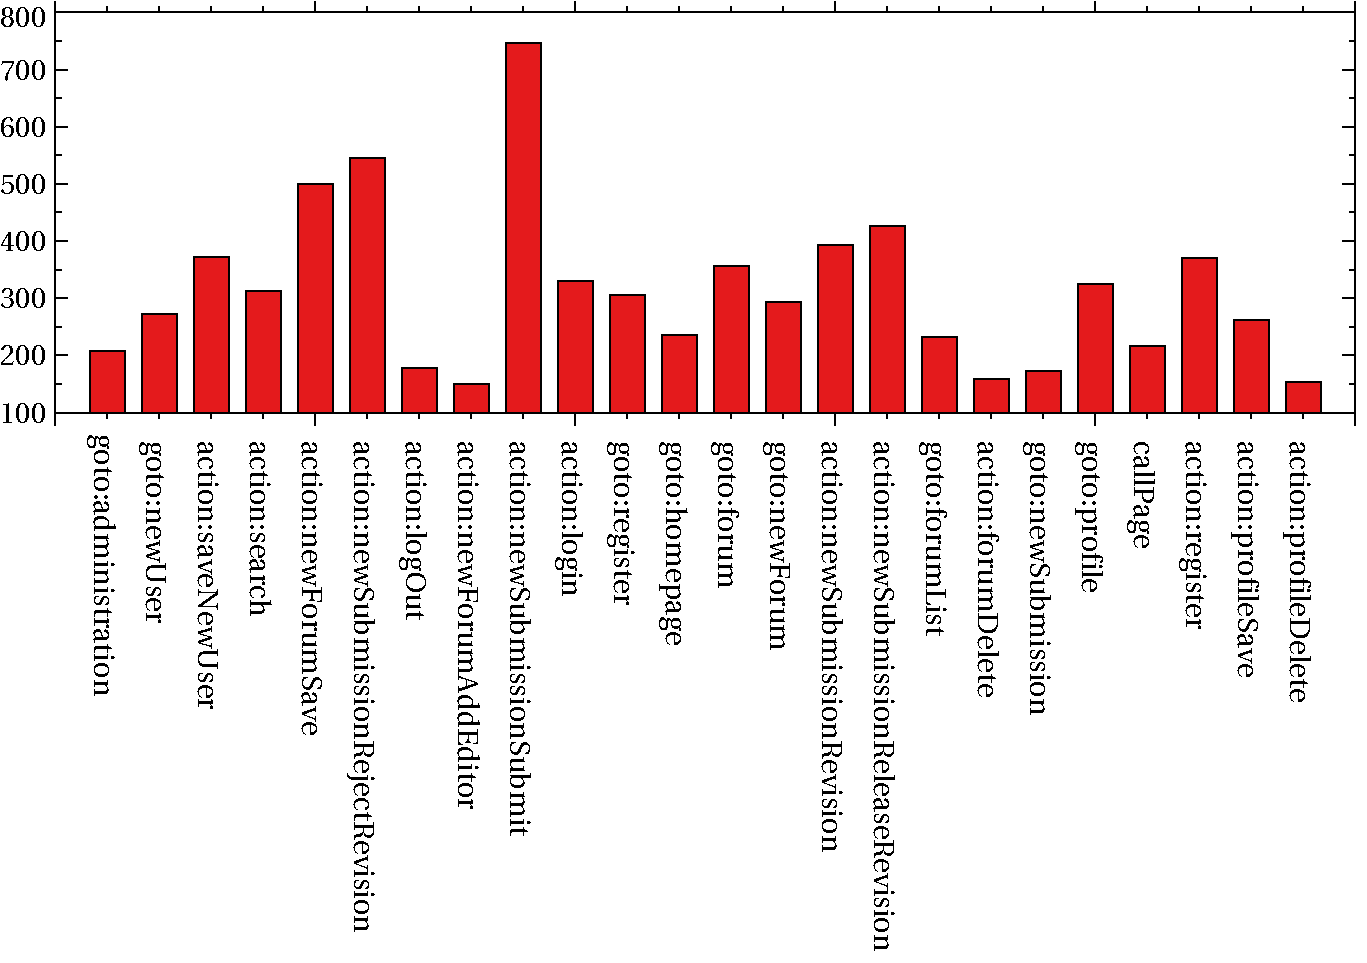
\includegraphics[width=\linewidth]{graphics/30worstcase.pdf}
	\caption{Konfiguration 1}
	\label{fig:worst30}	
\end{figure}
\begin{figure}[H]
	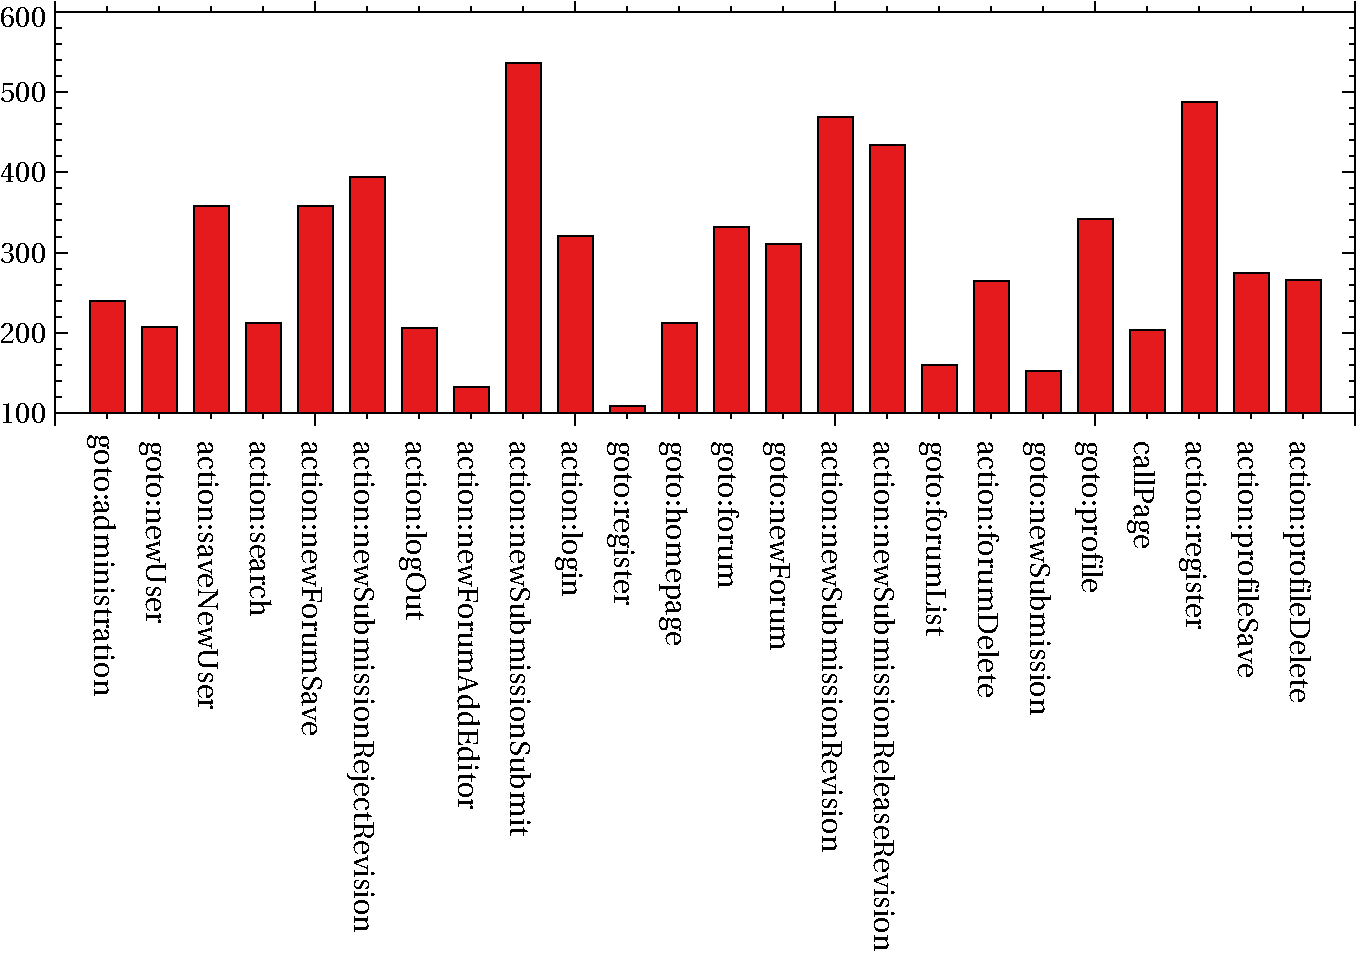
\includegraphics[width=\linewidth]{graphics/50worstcase.pdf}
	\caption{Konfiguration 2}
	\label{fig:worst50}	
\end{figure}

In \hyperref[fig:boxplot]{Abbildung 2} sieht man einen Boxplot, der die Werte der zwei Konfigurationen vergleicht. Im Boxplot zeigen die Whisker das 9/91 Perzentil. Der Kreis in der Box ist jeweils der Mittelwert.

\begin{figure}[H]
	\includegraphics[width=\linewidth]{graphics/boxplots.pdf}
	\caption{Boxplot}
	\label{fig:boxplot}	
\end{figure}


\subsection{Interpretation}

\subsection{Einschränkungen}
